\def\code#1{\mbox{\texttt{#1}}}


\chapter{Recurrent Convolutional Neural Network}
by Patrick Dammann

\bigskip

This chapter of the project will focus on an attempt using a model, that combines convolutional layers followed by a recurrent layer with preprocessing based on fourier transformation.

\section{Related Work}
\label{sec:rcnn-related}
The model used in this chapter was proposed by a blog post
\footnote{http://deepsound.io/music\_genre\_recognition.html}
by DeepSound, where they used it on the GTZAN \cite{1021072} dataset. Here, we try to adapt their method and applying that model to a bigger dataset.

The main idea of the model is based on convolutional neural networks (where it is hard to choose any the right papers to mention), and LSTMs \cite{Hochreiter:1997:LSM:1246443.1246450}, which are a special form of recurrent layers.

A blog post \footnote{http://benanne.github.io/2014/08/05/spotify-cnns.html} by a spotify intern uses a similar approach.

\section{Mel Spectrograms / Preprocessing}
\label{sec:rcnn-mels}

This approaches main attempt was to analyse sound in a similar way to humans. Since we humans perceive sounds as individual tones, but then give them a new meaning when they are combined in the right way, at the same time as well as in a sequence. Our hearing uses cells, that perform a frequency decomposition: this can easily be simulated via a discrete fourier transformation, since our data is present in discrete data points. To be able to analyze individual or consecutive tones, we need to analyze short, overlapping windows of the music to be sure that things that humans would consider a single sound is caught. This technique is called the Short Time Fourier Transform (STFT), which does a fourier transformation for each sliding window. The paper assumes that the shortest, distinguishable sound is about 10ms long, which would be near to $2048$ samples at $22050$Hz sampling rate(~0.0929ms), so we use this as the window size, while using $1024$ as the stride, to enforce an overlap of $50\%$ between two adjacent windows.

\begin{minipage}{1.0\textwidth}
\[
    stft(m, \omega)=\sum^{\infty}_{n=-\infty}s[n]w[n-m]e^{-i \omega n}
\]
\[
    x := \text{sampled signal}
\]
\[
    w := \text{window function, that is $1$ for selected window, $0$ otherwise}
\]
\vspace{1cm}
\end{minipage}

\begin{figure}
    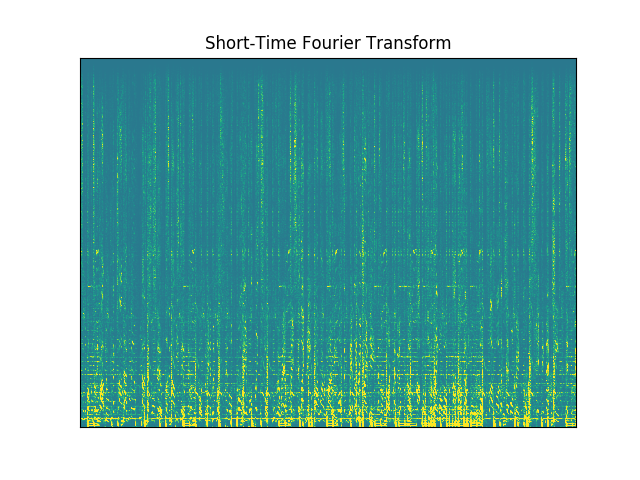
\includegraphics[width=0.5\textwidth]{{images/pepe/stft}.png}
    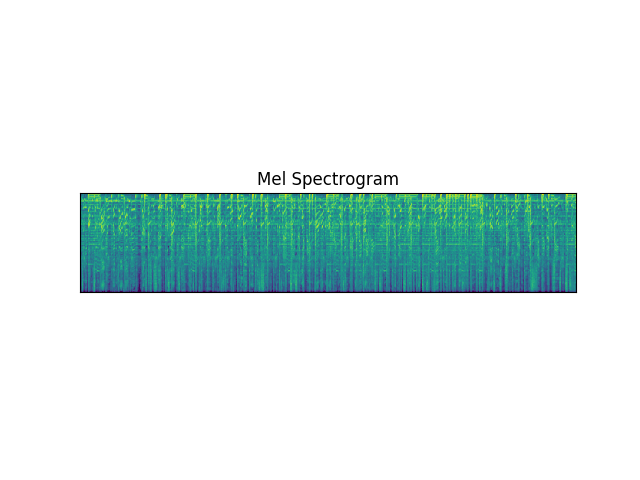
\includegraphics[width=0.5\textwidth]{{images/pepe/mel}.png}
\caption{\label{fig:rcnn-mels}Here, we see the difference between the Short-Time Fourier Transformation (\emph{left}) and the Mel spectrogram (\emph{right}). Primary, the difference in the dimensionality (through the binning) can be seen immediately, while the other advantages are not to be spotted by the naked eye. Both visualizations have in common that they plot the frequency domain on the y-axis and the time domain on the x-axis.}
\end{figure}


A Mel spectrogram is basically the same thing, but converts frequencies to Mel scale (a unit that tries to map equal distances to tones, that humans perceive as equally distanced), and then sums them up to a given number of bins.
We use $128$ bins for our spectrogram, since the hearable spectrum ranges from ~16HZ to  ~19,000Hz, which are $~10.2$ octaves, which are $~123$ tones, so we should be catching everything that gathers around the "main frequencies in the traditional tone ladder" as a single feature.

An optical comparison between the two is provided in figure \ref{fig:rcnn-mels}.

\section{The Model}
\label{sec:rcnn-model}

\begin{figure}
    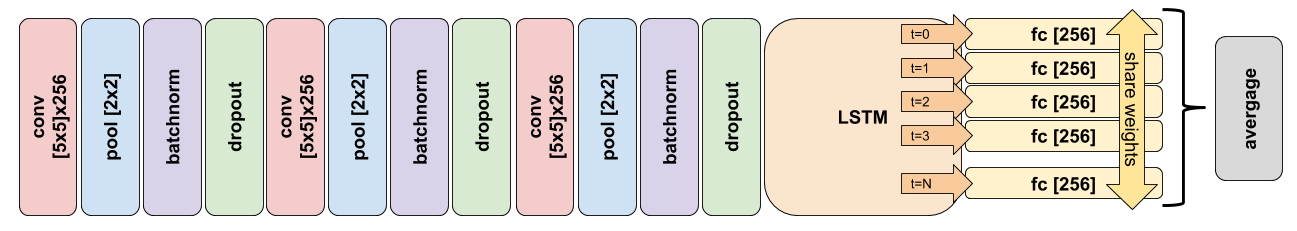
\includegraphics[width=1.0\textwidth]{{images/pepe/model}.png}
\caption{\label{fig:rcnn-model}This is the used model architecture. The model starts with it's convolutional layers (together with their usual companions), followed by an LSTM and a time-distributed fully connected layer, over whose scores is averaged unweighted.}
\end{figure}

The first part of the network consists of convolutional layers. Since tones in all frequencies can be combined to create a hearing experience, it makes sense to consider the frequency domain as feature axis, so the \mbox{\texttt{Conv1D}} layers' filters are two-dimensional and shifted along a single axis, the time axis. This way, information about different frequency bins can be combined over a short amount of time in each laver. Around the convolutional layers, which utilize \code{ReLU} activations, there are \code{BatchNorm}, \code{Pooling} and \code{Dropout} layers.
A visualization of the model can be seen in figure \ref{fig:fig:rcnn-model}.

The next part is a \mbox{\texttt{LSTM}}, which is a special form of a recurrent layer. LSTM cells carry a state and have several weight matrices that, dependent on state and input, give out instructions on how to alter the state as well as an output.
Therefore, LSTMs are used to analyze sequences, since the state allows them to combine information over very long signals and to treat features differently dependent on their predecessors. This is why we then feed the individual feature vectors for each discrete time step into the LSTM, and apply a fully connected layer to the output of each. This fully connected layer has the same weights for each time step.
DeepSound argue that e.g. a rock song should sound like a rock song at every part of the song. Another reason why this might be a good idea is that this way, the gradient should vanish a lot less during backpropagation, since each step in the LSTM is considered for the final result. 

\section{Initial Pre-Processing}
\label{sec:rcnn-pre-proc}
Since the dataset is huge and the song's durations vary strongly, random crops of the song were used, which have been turned into mel spectrograms by the \emph{pytorch} \mbox{\texttt{Dataloader}} on demand. During this approach, training epochs have needed too much time to train many of them, which is why benchmarks of the proportion of data preprocessing time to training time have been made.\todo{plot or table}
Based on these measurements and the opinion that the gain in time is definitely worth the additional needed space, all data is then pre-processed by a script before training, which creates mel spectrograms for all full songs and saves them on hard disk. During training, files are loaded from disk and cropped randomly with a fixed size along the time axis. 

\section{First Training}
\label{sec:rcnn-first}

\begin{figure}
    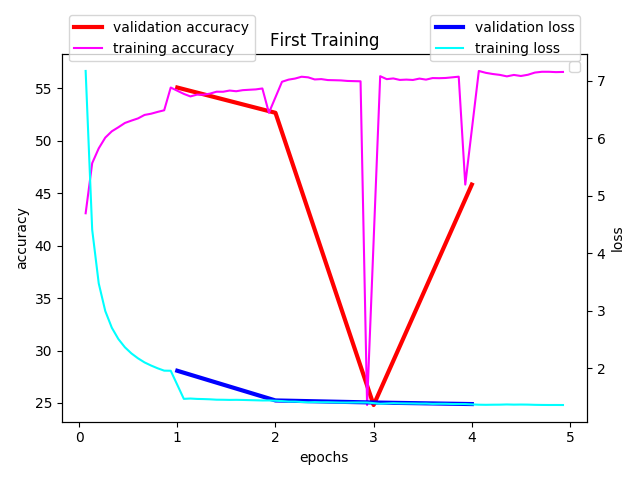
\includegraphics[width=0.5\textwidth]{{images/pepe/logs1.p}.png}
    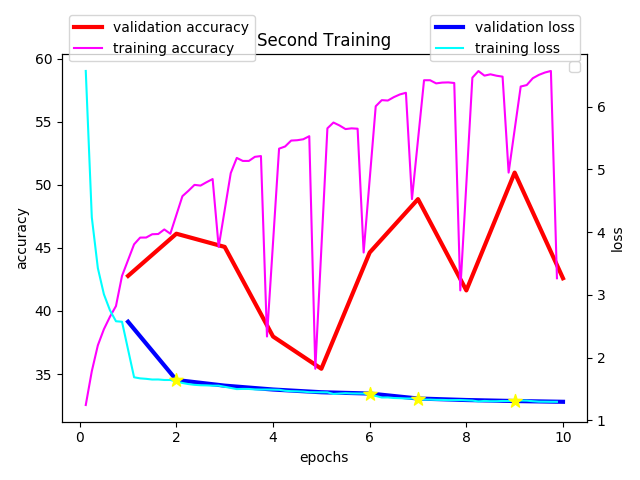
\includegraphics[width=0.5\textwidth]{{images/pepe/logs2.p}.png}
    \caption{\label{fig:rcnn-train} On the left, one can see the training progress of the first session. The validation accuracy is not stable at all and does not reach anywhere near acceptable results. The training has been canceled early.\\
    On the right, the second session is plotted. The validation accuracy seems a lot more stable than before, which might be thanks to the filtered dataset. The yellow stars denote a reduction of the learning rate to one third.}
\end{figure}

The first training was continued over $4$ to $5$ epochs, but then canceled, since we found problems with the data, as mentioned in chapter \todo{uncomment}%\ref{dataset}.
The data shown in figure \ref{fig:rcnn-train} is included to show the difference to further training sessions.
With $~53.5$\% of the songs that seems to belong to all different kinds of genres being labeled with no label, the best achieved accuracy of $~55$\% is only slightly better than always guessing "no label", which the model does in XX\%\todo{fill in} of all cases.

\section{Second Training}
\label{sec:rcnn-second}
This training session has been made with the filtered dataset, where all songs without label have been removed. The validation accuracy here peaks at $~50$\%, which is better than the $~55$\% of the previous attempt, considering the structure of the dataset, but still worse than the $70+$\% achieved in the paper\footnote{But, they are only using $10$ genres instead of $16$}. We believe, that the unlabeled data in the dataset "confused" the network by training it to assign the empty label to songs, that should actually be categorized into on the other classes.

\section{Third Training}
\label{sec:rcnn-third}

\begin{figure}
    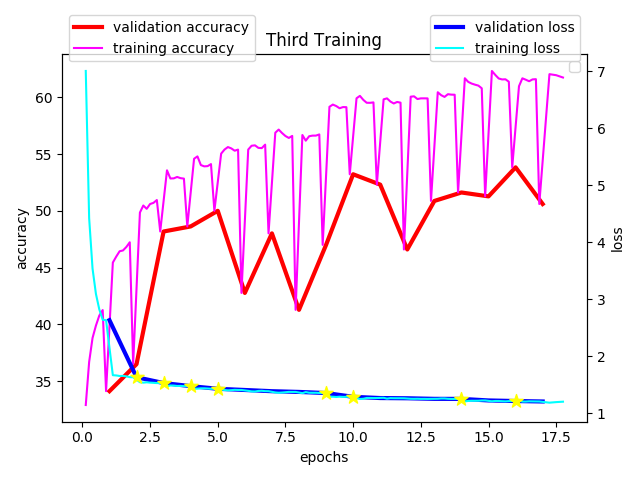
\includegraphics[width=0.7\textwidth]{{images/pepe/logs3.p}.png}
    \caption{\label{fig:rcnn-train2} This session showed the so far most stable and best accuracies and losses achieved during the third training session, with $~53$\% peak accuracy on the filtered dataset.}
\end{figure}

In a follow-up experiment, the performance was tried to be improved by Xavier/2 weight initialization\cite{pmlr-v9-glorot10a} and longer training time. The model itself has not been altered. The results have been plotted into figure \ref{fig:rcnn-train2}.

\section{Including a Visualizing Bottleneck}

\begin{figure}
    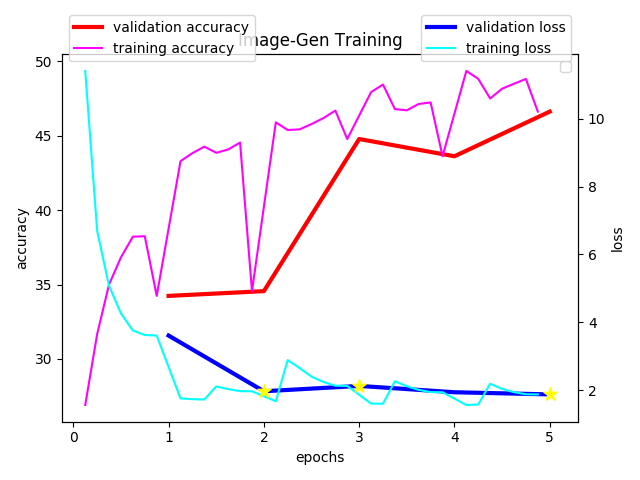
\includegraphics[width=0.45\textwidth]{{images/pepe/logs4.p}.png}
    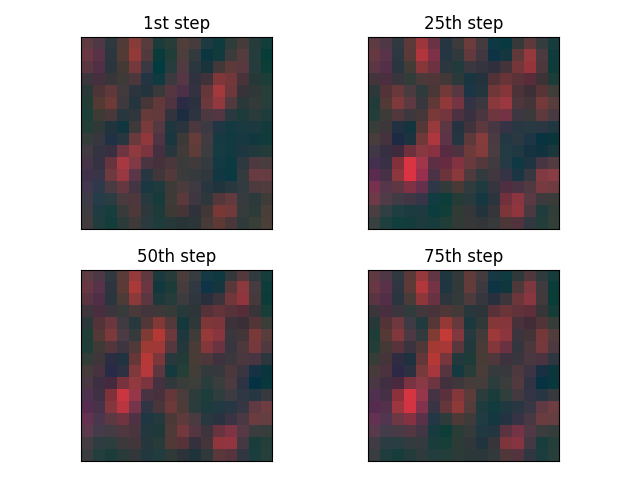
\includegraphics[width=0.25\textwidth]{{images/pepe/image_gen_1}.png}
    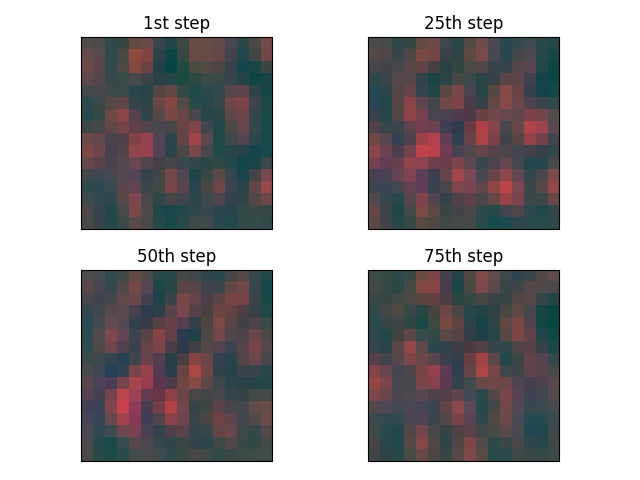
\includegraphics[width=0.25\textwidth]{{images/pepe/image_gen_2}.png}
    \caption{\label{fig:rcnn-gen} The training session on the altered model went well, what the stable accuracy in the left plot shows. Yellow stars are again indicating a scheduling of the learning rate.\\
    On the right are images sampled from two different rock songs. While small differences can be seen, the main hot spots appear at the same places. Unfortunately, all values resolved around zero before the tanh, which is why these images have been mostly grey and had to be boosted in contrast to be viewable and representable with 24bit color depth.}
\end{figure}

Out of interest, the following step was to alter the model in a way that it would not only classify music, but also be able to generate visualizations for music that resembles it in a way learned by the model. The approach taken here to achieve this is to add time-distributed convolutional layers between the LSTM and the time-distributed linear layers, that would create something that could be resembled as an image. Realizing this was easy by reshaping the outputs of the LSTM to squares with shape $16x16$ and then applying convolutional layers with only three filter banks to them. Afterwards, the resulting "image" is additionally blurred with a gaussian filter to make the image look less aliased by decreasing difference and increasing dependence between adjacent pixels.\\
When a visualization is about to be extracted from the network, the song is put in and for each time step the resulting image is returned. For being able to interpret the result as an image, an additional tanh-layer is applied, so all values lie between $0$ and $1$.\\
Adding the image generation layers did not decrease accuracy much, but definitely notable, with a new maximum of $~46.5$\%, but the stability of the validation accuracy suggests that more epochs could have generated better results. An example for visualizations generated by the model can be seen in figure \ref{fig:rcnn-gen}, together with a plot of the training process.